\begin{frame}
\frametitle{Task 1: Theory}
If the dipole is considered to be short
\begin{equation}
\mathbf{G}(\theta, \phi) = G_{\theta}\hat{\theta} + G_{\phi}\hat{\phi},
\end{equation}
with

\begin{equation}
\begin{cases}
&G_{\theta} = G_{\theta}(\theta, \phi) = C_k\eta I_0 l/2cos(\theta)sin(\phi)2jsin(khcos(\theta))) \\
& G_{\phi} = G_{\phi}(\theta, \phi) = C_k\eta I_0 l/2cos(\phi)2jsin(khcos(\theta))).
\end{cases}
\end{equation} 
with 
\begin{equation}
\begin{cases}
& C_k = -jk/4\pi \\
& \eta \approx 120 \pi [\Omega] \\
& k = \frac{2*pi}{\lambda} \\
& h = \frac{\lambda}{4}\\
& I_0 = \text{incident current}
 \end{cases}
\end{equation}


\end{frame}

\begin{frame}
\frametitle{Task 1: Results}
\begin{figure}[h]
\centering
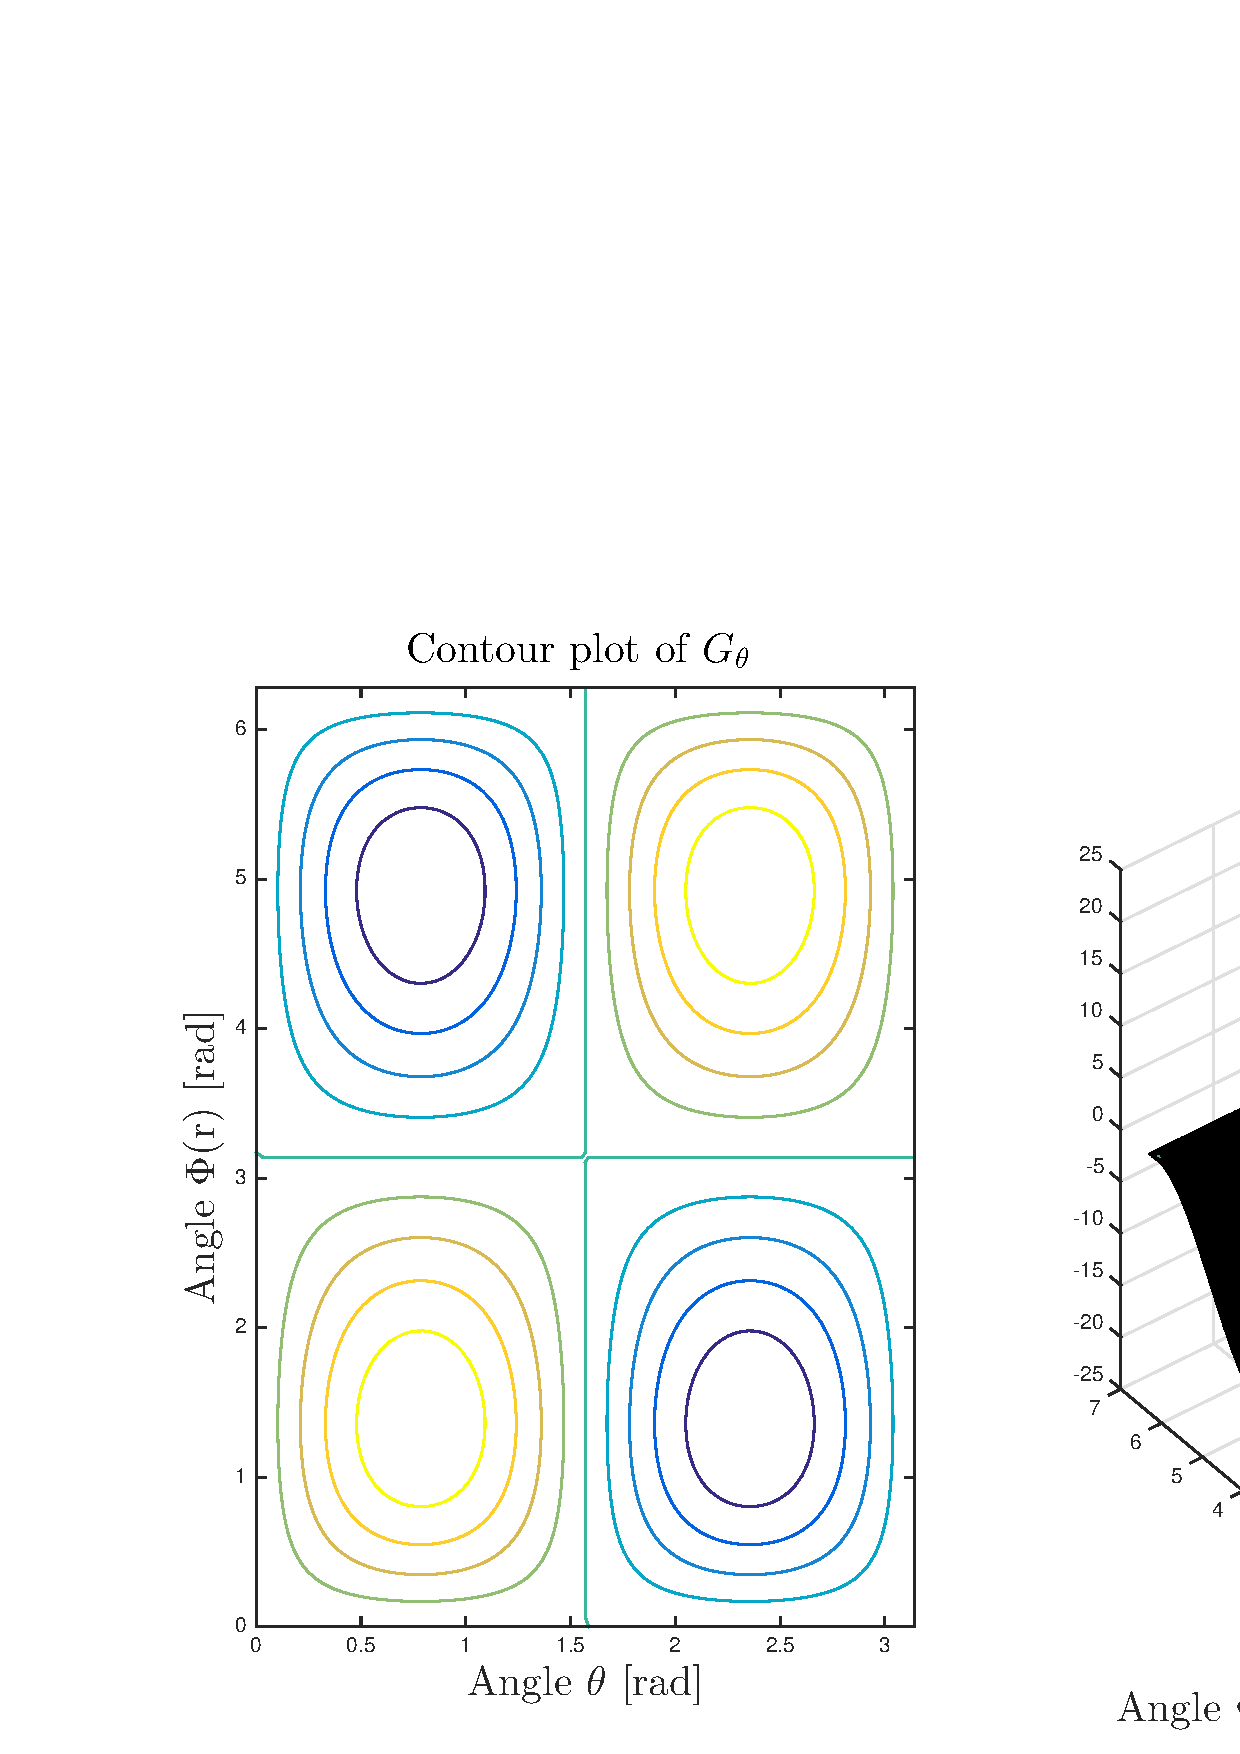
\includegraphics[scale=0.3]{/Users/marikasvensson/Documents/MATLAB/MicroProject/finished/task1/Gth.png}
\caption{This figure shows $G_\theta$ as a function of $\theta$ and $\phi$}
\label{task1:Gth}
\end{figure}

\end{frame}

\begin{frame}
\frametitle{Task 1: Results}
\begin{figure}[h]
\centering
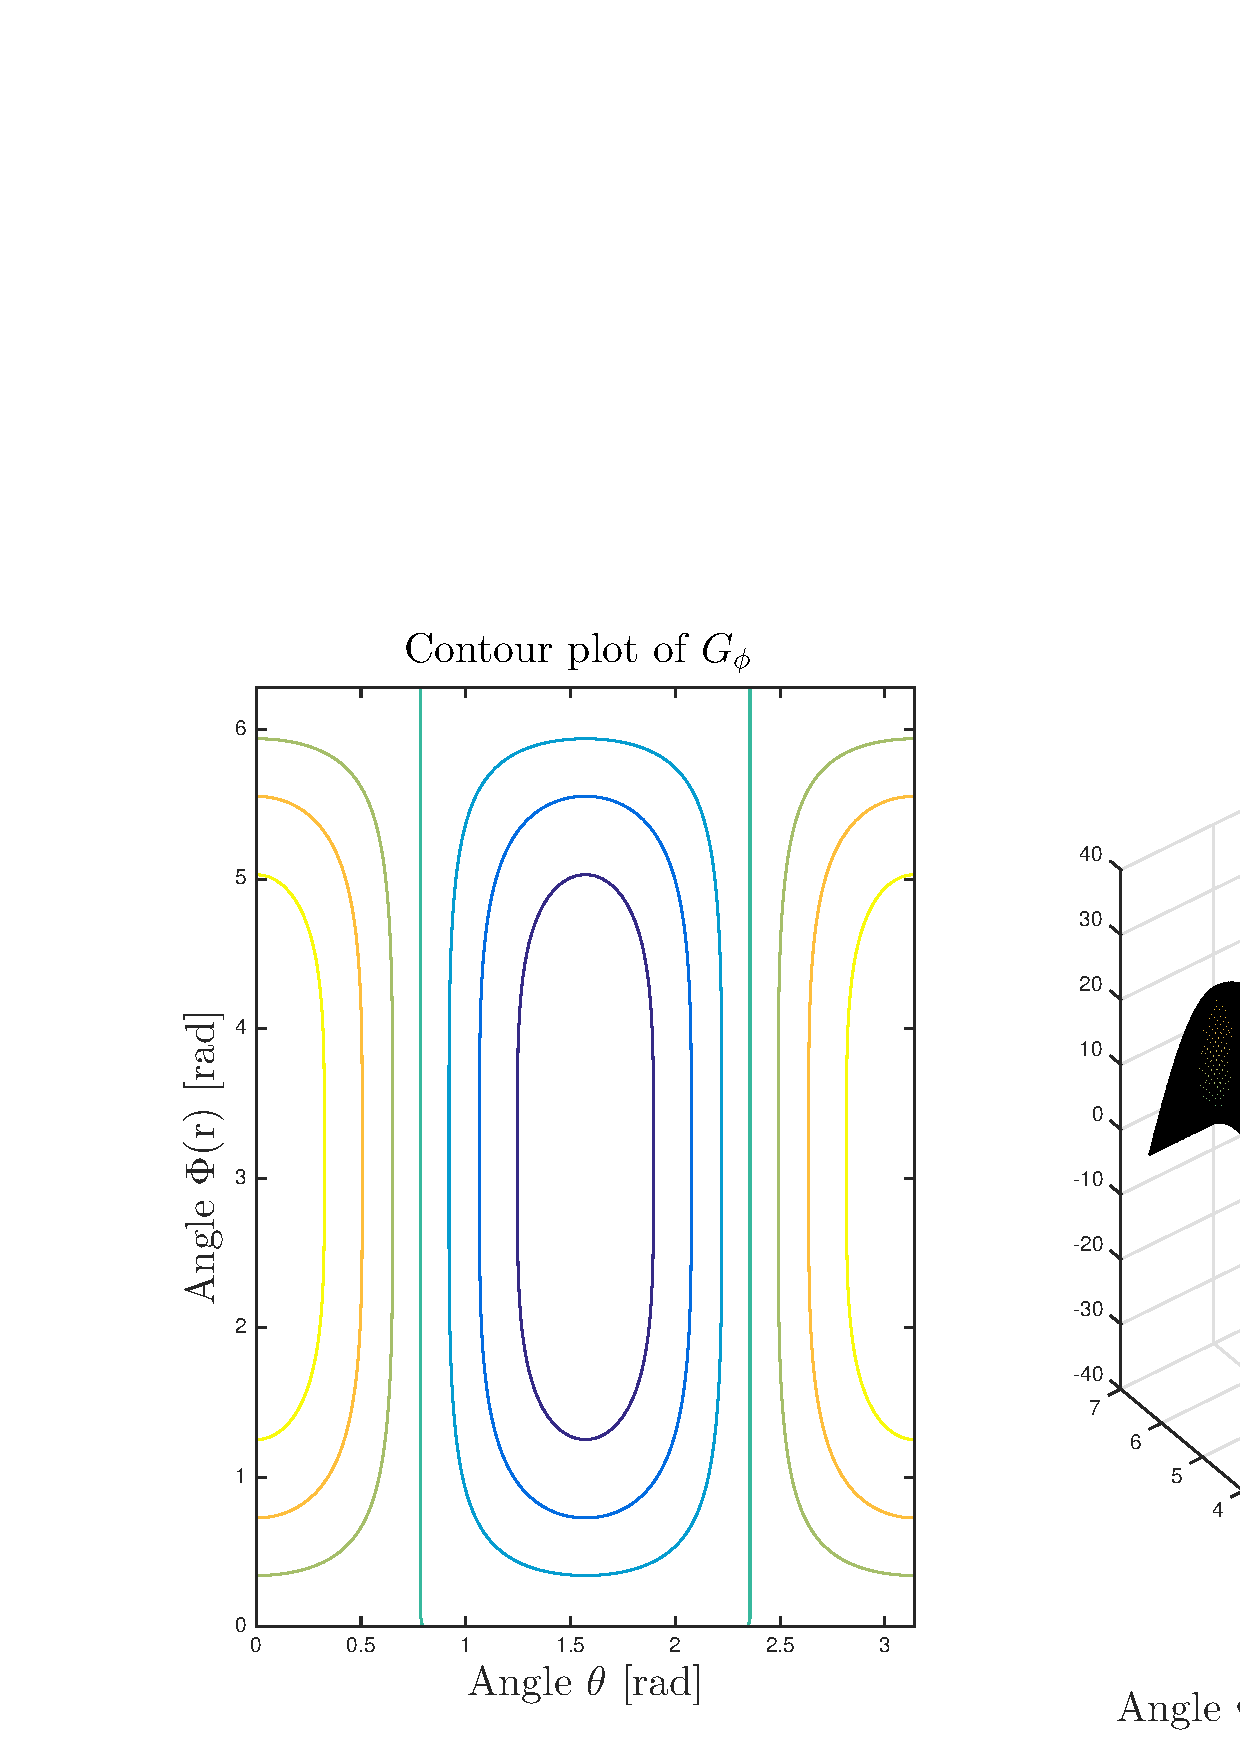
\includegraphics[scale=0.3]{/Users/marikasvensson/Documents/MATLAB/MicroProject/finished/task1/Gphi.png}
\caption{This figure shows $G_\phi$ as a function of $\theta$ and $\phi$}
\label{task1:Gphi}
\end{figure}
\end{frame}